\documentclass[10pt]{article}

\usepackage{graphicx}
\usepackage{natbib}
\usepackage[hyphens]{url}
\usepackage{color}
\usepackage{times}
\usepackage{verbatim}
\usepackage{amsmath}
\usepackage{enumitem}
\usepackage[hidelinks,breaklinks=true]{hyperref}
\usepackage[margin=1in]{geometry}
\usepackage{float}
\usepackage{caption}
\usepackage{animate}
\usepackage[backend=biber, style=authoryear]{biblatex}
\addbibresource{references.bib}

\renewcommand\labelenumi{(\roman{enumi})}
\renewcommand\theenumi\labelenumi

\title{Examining the Effects Climate Change across the Globe}

\author{Adelynn Shirts \and Spencer DenBleyker \and Zayne Maughan}

\begin{document}

\renewcommand{\topfraction}{1.0}
\renewcommand{\bottomfraction}{1.0}
\renewcommand{\textfraction}{0.0}
\renewcommand{\floatpagefraction}{1.0}
\renewcommand{\dbltopfraction}{1.0}


\maketitle

\begin{abstract}
The project analyses global climate change using data from the IMF's Climate Change Dashboard. We examine 4 key datasets: surface temperature change, mean sea level change, climate-related disasters, and forest and carbon levels. By creating and analyzing different visualizations we found a concerning trend: the world is getting hotter and wetter. We are seeing more climate-related natural disasters and less forest coverage.  
\end{abstract}

{\small
\noindent\textbf{Keywords:}
climate change, global warming, climate change analysis, deforestation, natural disasters, sea level rise, environment, environmental data analysis, climate visualization}



%%%%%%%%%%%%%%%%%%%%%%%%%
\section{Introduction}
\label{Introduction}
%%%%%%%%%%%%%%%%%%%%%%%%%
Climate change is one of the most pressing and urgent issues of our time, affecting economies, ecosystems, and millions across the globe. In response to the Call of the Data Analysis competition, we explored key visualizations that illustrate the multifaceted effects of global climate change. We focused on four major indicators--global temperature change, sea level changes, the frequency and severity of climate-related disasters, and forest coverage and carbon levels. By analyzing these visualizations, we hope to gain a better understanding of how these interconnected phenomena drive global climate change and highlight the importance of monitoring and mitigation strategies. We will begin by looking at the yearly average surface temperature change and the average sea level change. After, we will explore climate-related disasters and how forest coverage and carbon levels have changed. 


%%%%%%%%%%%%%%%%%%%%%%%%%
\section{Global Temperature Change}  
\label{TempChange}
%%%%%%%%%%%%%%%%%%%%%%%%%
To understand the progression of climate change over time, we began by analyzing a dataset of yearly average surface temperature changes across countries from 1961 to 2022 in degrees Celsius. Specifically, the data reflects the year-over-year change in temperature for each country, relative to the previous year. This dataset contained some missing values that required careful removal or imputation. Some countries, mainly in the Soviet bloc, had missing data for the earliest reported years in this dataset. For these countries, we computed continent-level average annual temperature change and used the reverse cumulative sum of these values to estimate plausible backfill values for each country, anchoring them to the first observed value for that country. We also enforced a constraint such that no value could fall below the observed minimum temperature change for each continent. For any internal missing data, we applied linear interpolation based on the already known yearly values. By following these steps, we were able to preserve the majority of the dataset, allowing for a more complete picture of the yearly global surface temperature change. 

\begin{figure}[H]
    \centering
    \begin{minipage}{0.48\textwidth}
        \centering
        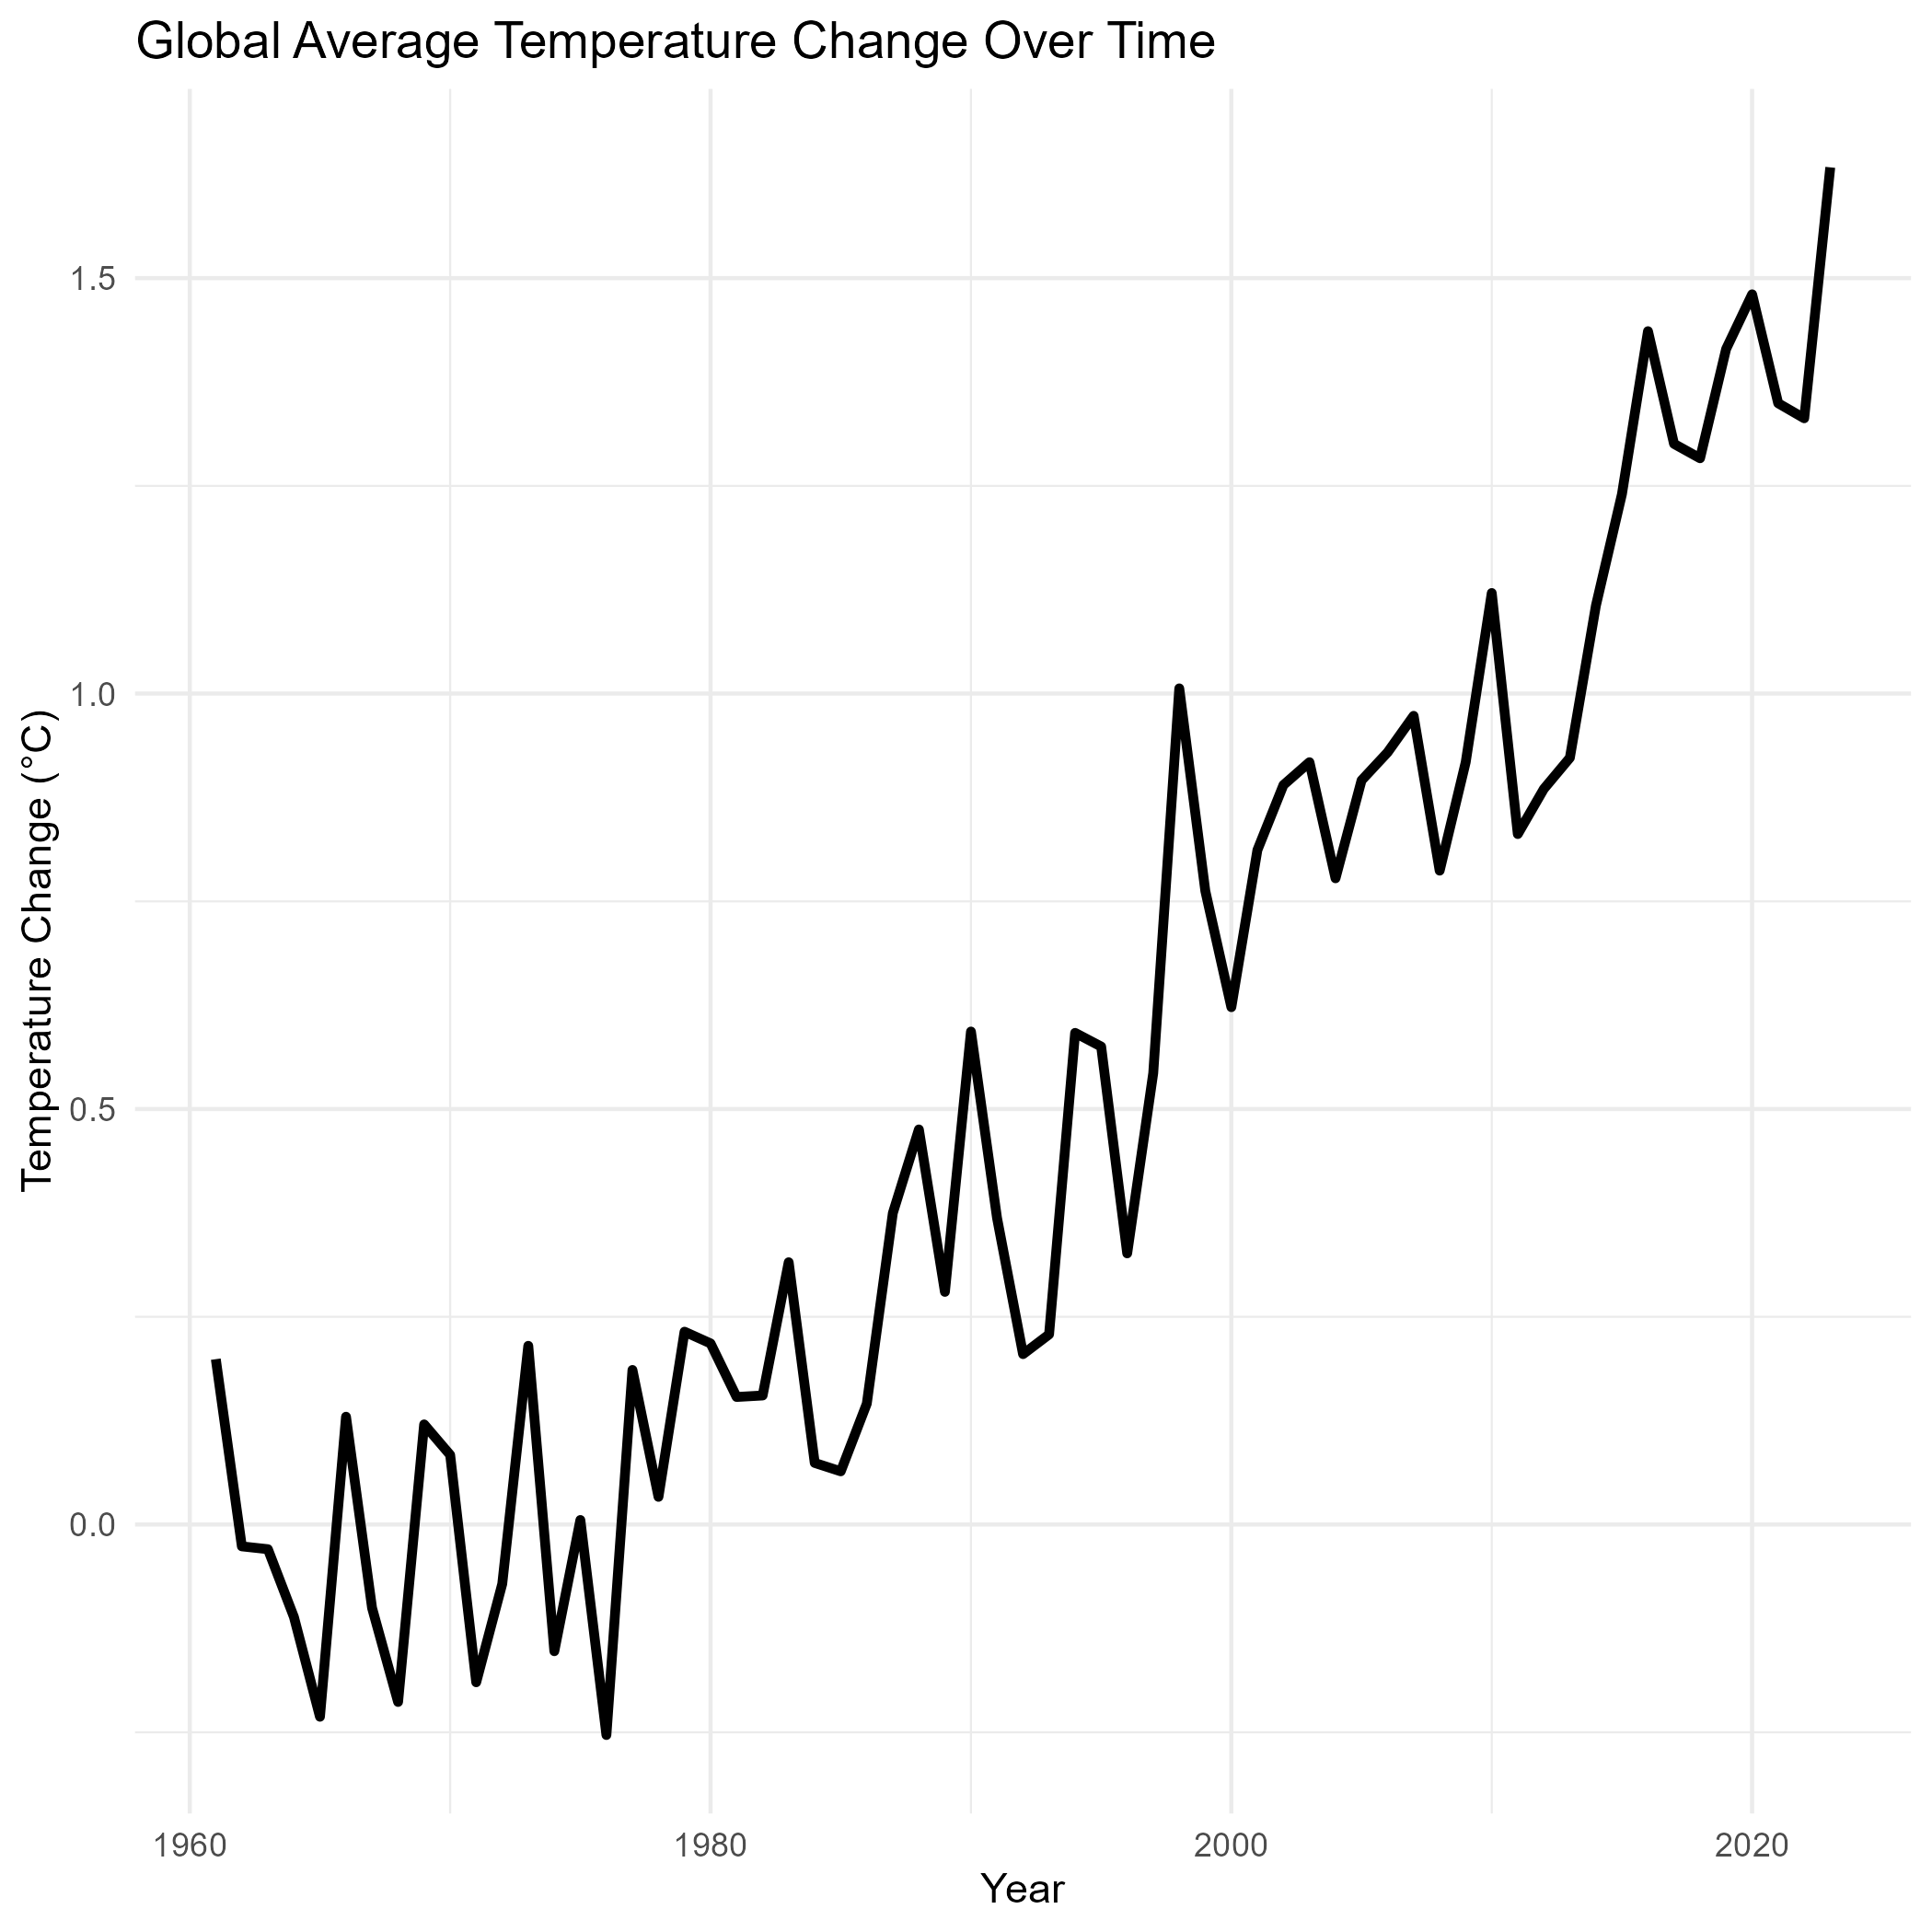
\includegraphics[width=\linewidth]{TempLine.png}
        \caption{Global average annual temperature change from 1961 to 2022. A clear upward trend can be seen, especially in recent decades.}
        \label{fig:lineplot}
    \end{minipage}
    \hfill
    \begin{minipage}{0.48\textwidth}
        \centering
        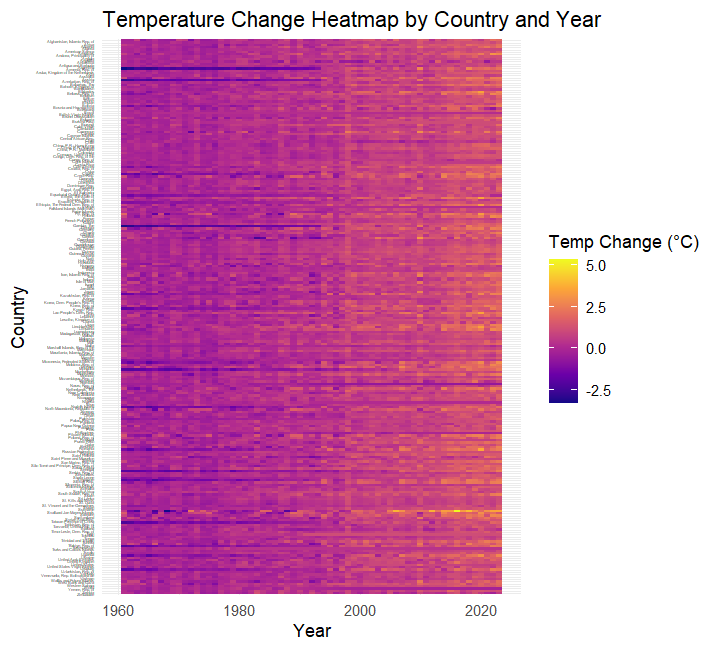
\includegraphics[width=\linewidth]{GlobalHeat.png}
        \caption{Heatmap showing yearly surface temperature changes across countries. Warmer colors indicate higher temperature changes.}
        \label{fig:heatmap}
    \end{minipage}
\end{figure}



%%%%%%%%%%%%%%%%%%%%%%%%%
\section{Sea Level Changes}  
\label{SeaChange}
%%%%%%%%%%%%%%%%%%%%%%%%%
The impact of rising temperatures can first be seen in the changing of sea levels. To do so, we looked at a dataset that ranged from 1992 and span over 30 years to 2025. This dataset, unlike the others, did not have supporting regions for the data and it mainly had just the individual seas themselves. There was some preliminary cleaning, including dropping some Na values from the set. This was done to ensure that missing years did not impact the analysis. Other than this no other changes were made to the data. As we see from the following pictures, the rising global temperature has also shown an increase in global sea levels. This can be seen in both figures shown below. 

\begin{figure}[H]
    \centering
    \begin{minipage}{0.48\textwidth}
        \centering
        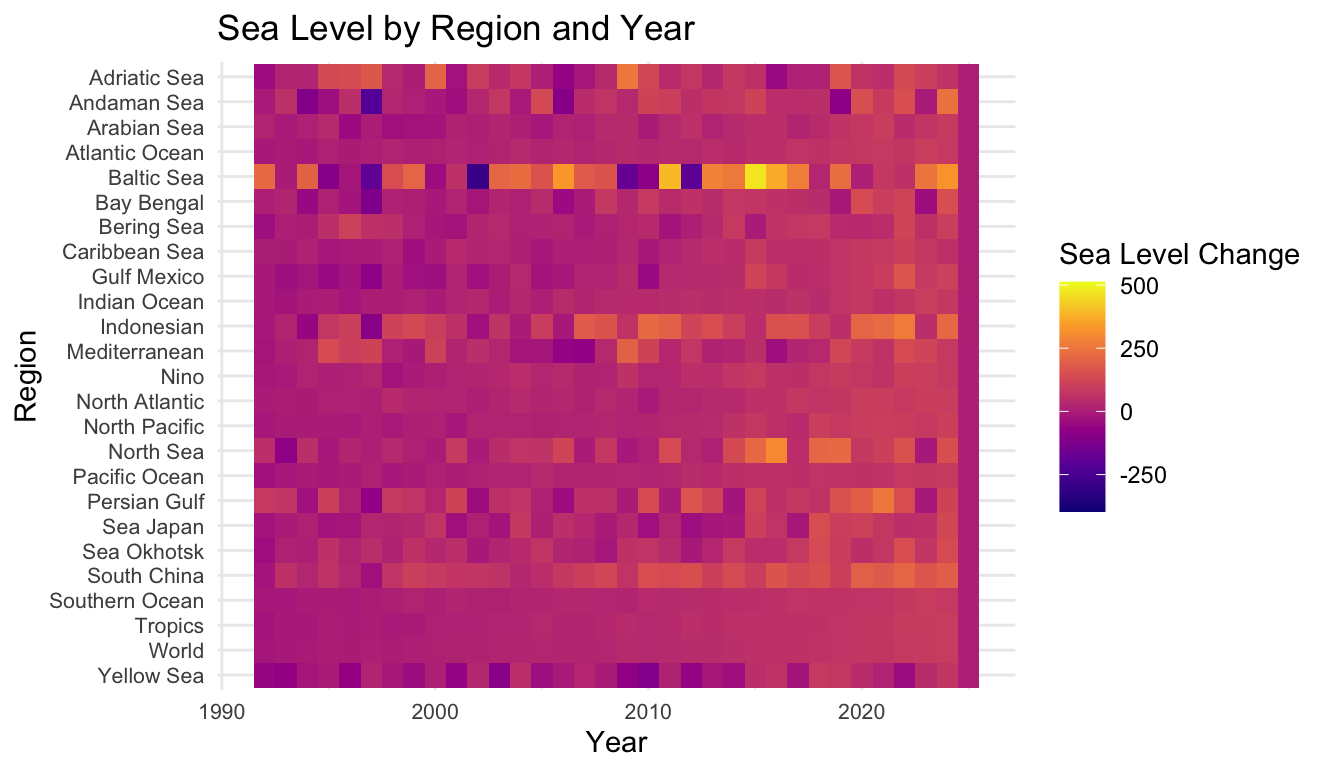
\includegraphics[width=\linewidth]{Sea_level_changed_x.png}
        \caption{Heatmap showing yearly sea levels.}
        \label{fig:sealevelheat}
    \end{minipage}
    \hfill
    \begin{minipage}{0.48\textwidth}
        \centering
        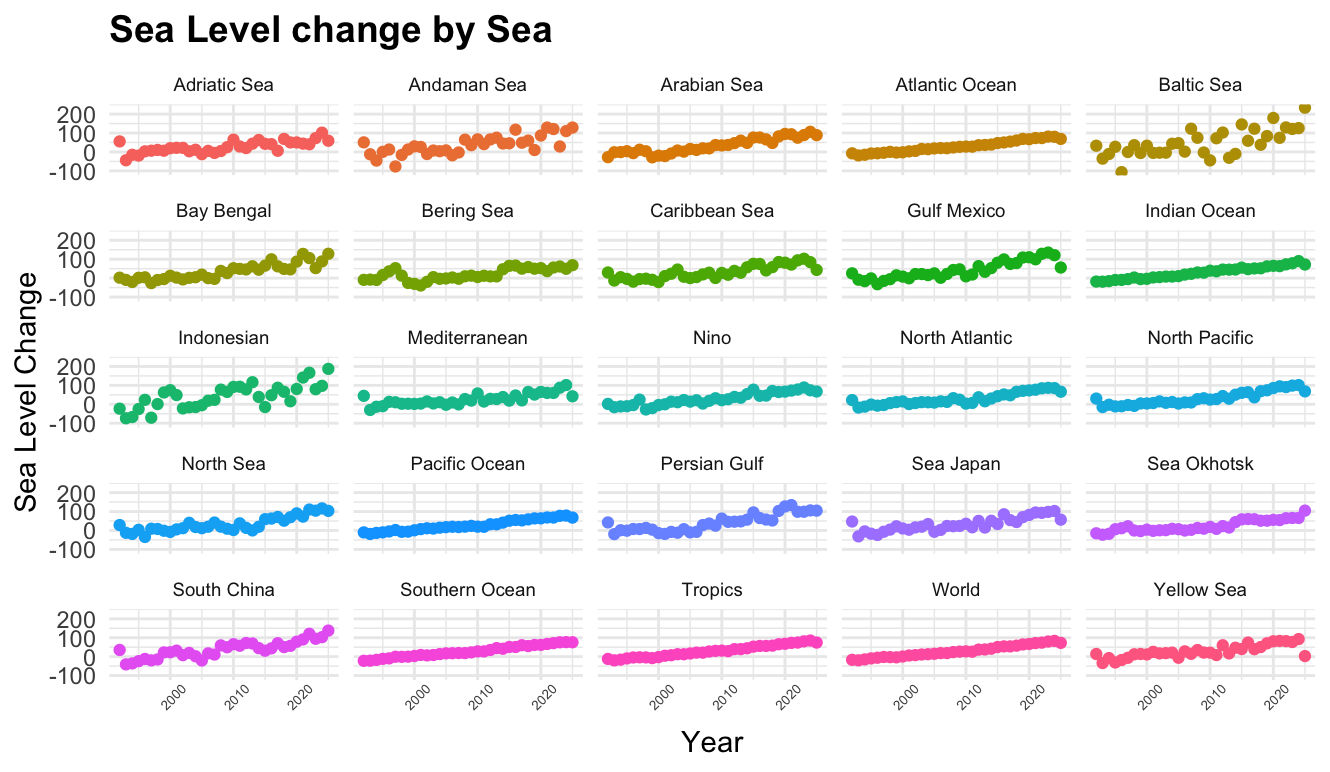
\includegraphics[width=\linewidth]{Sea_level_dot_x.png}
        \caption{Dot plot showing yearly sea levels across different seas.}
        \label{fig:sealeveldots}
    \end{minipage}
\end{figure}



%%%%%%%%%%%%%%%%%%%%%%%%%
\section{Climate-Related Disasters}  
\label{Disasters}
%%%%%%%%%%%%%%%%%%%%%%%%%
To understand the number of disasters over time, we analyzed a dataset of different types of disasters across countries from 1988 to 2022. Specifically, the data looks at droughts, hot temperatures, floods, landslides, storms, wildfires, and the total number of disasters for each country. The original data set only contains countries and not continents, as well as having all seven types of disaster for each row. We first cleaned the data, removing any unnecessary columns, adjusting the column names of the years to remove an "F" from the beginning of each year column, and summed up the disasters by continent, using the country codes to combine them. The continents that we divided them into are Africa, the Americas, Asia, Europe, and Oceania. Next, we split the data by disaster type. Then, so that we could analyze the trends more easily, we averaged the number of disasters by decade.

\begin{figure}[H]
    \centering
    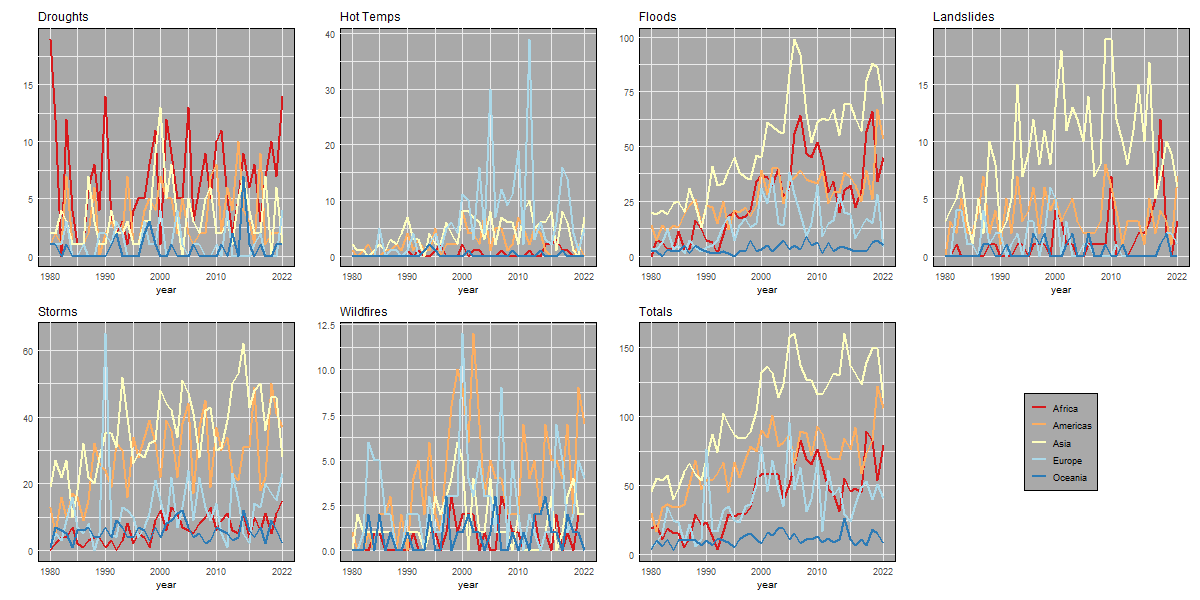
\includegraphics[width=0.8\textwidth]{Continent_Disasters.png}
    \caption{The number of disasters by continent by year.}
    \label{fig:disast_year}
\end{figure}



\begin{figure}[H]
    \centering
    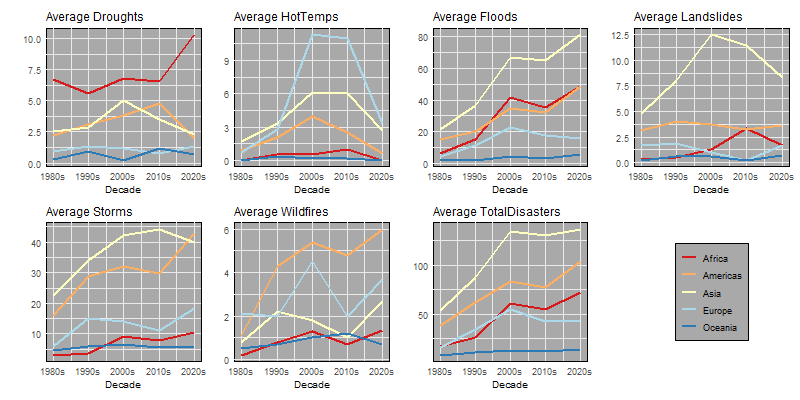
\includegraphics[width=0.8\textwidth]{Decade_disasters.png}
    \caption{The number of disasters by continent by decade. A clear upward trend in the total number of disasters can be seen.}
    \label{fig:disast_decade}
\end{figure}
As shown in Figure~\ref{fig:disast_year} and Figure~\ref{fig:disast_decade}, we can see that different continents seem to struggle with different types of disasters. Africa struggles with droughts, which makes sense due to all of the deserts. The Americas struggle with wildfires, and in the 2020s, they struggled with storms. Asia struggles with floods, landslides, and storms, which makes sense since stronger storms can bring floods and destabilize the ground, which can bring landslides. Europe struggled with hot temperatures for the last three decades, but not much else. Oceania did not get many disasters at all, being at or near the bottom every decade. There are some years in which one continent goes above another, such as Europe a few times throughout the years, such as with storms around 1990, and wildfires around 2000.


%%%%%%%%%%%%%%%%%%%%%%%%%
\section{Forests and Carbon}  
\label{ForestCarbon}
%%%%%%%%%%%%%%%%%%%%%%%%%
This is the area that might not be directly causally related to the rise in temperatures. Rather, this might contribute to these temperatures. Looking at the data, it spans the period of 30 years from 1992 to 2022. We wanted to see how deforestation has affected countries around the world. To do this, we put the average forest area per country on the log scale to get a better relative baseline to view across the globe. However, we removed Qatar as it does not have any forest area, and the log of zero is undefined. When doing this, we saw certain countries moving faster than what we expected. After further review, we determined that a better metric would be the average percentage of forest area over hectares. We therefore transformed the data and came up with the following graphic to better visualize how deforestation has affected countries around the world.

\begin{figure}[H]
    \centering
    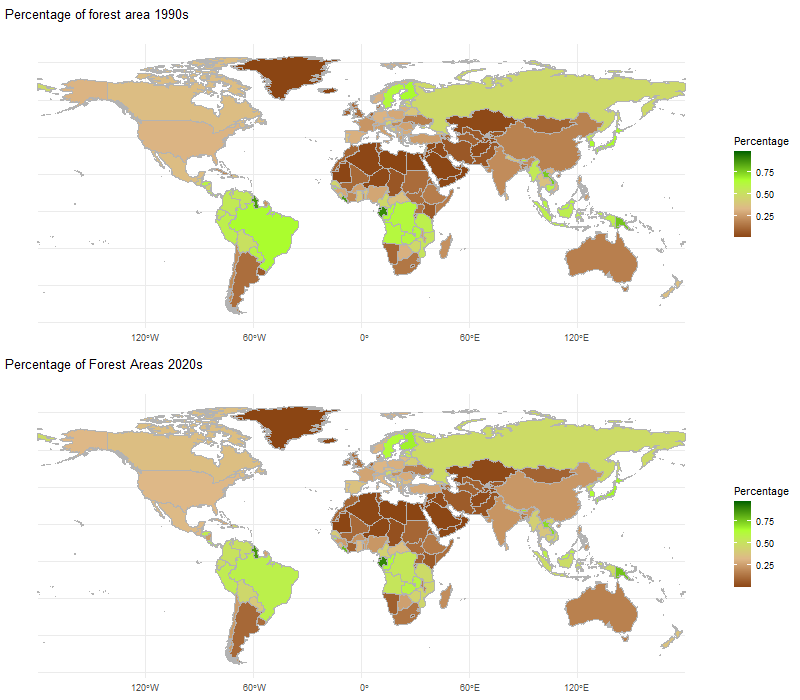
\includegraphics[width=0.8\textwidth]{forest_pct.png}
    \caption{The average percentage of land area covered by forests in the 1990s and 2020s. A few countries can be seen to have lower percentages in the 2020s.}
    \label{fig:forest_pct}
\end{figure}

Looking at Figure~\ref{fig:forest_pct}, we see that the countries that seem to be the most effected are Brazil, Nicaragua, Myanmar, Cote d'Ivoire, and Malawi


%%%%%%%%%%%%%%%%%%%%%%%%%
\section{Conclusions and Outlook}  
\label{Outlook}
%%%%%%%%%%%%%%%%%%%%%%%%%
Climate change has shaped the planet in profound ways, and continues to do so. Our analysis across global temperatures, sea level changes, climate-related disasters, and forest coverage and carbon levels shows clear and concerning trends. The world is getting warmer, every country over. Sea levels are rising. The number os climate-related disasters is increasing year by year, affecting more and more communities across the globe. Deforestation is a major cause for concern. Continuing global cooperation, monitoring, and initiatives will help us push back against these distressing trends. Future work might include more advanced analysis by building predictive models to forecast changes in temperature, sea levels, and disasters. An interactive Shiny dashboard may give further insight into how different phenomena, such as temperature fluctuations and disasters, affect various regions and countries. 


%%%%%%%%%%%%%%%%%%%%%%%%%
\section{Acknowledgments and Work Distribution}  
\label{acknowledgments}
%%%%%%%%%%%%%%%%%%%%%%%%%
\textbf{Adelynn Shirts:} Adelynn chose the data and competition and wrote the proposal with suggestions from Spencer. Adelynn cleaned and visualized the temperature data. She also presented her sections of the presentation. Adelynn formatted the final paper and wrote the abstract, intro, temperature, and conclusion sections. She also assembled the bibliography and the GitHub repository.\\
\textbf{Spencer DenBleyker:}  Spencer chose the data and competition and gave suggestions for the proposal. He also did visualizations for the climate-related disasters and forest and carbon datasets. Spencer presented his sections of the final presentation. Spencer wrote the climate-related disasters section of the report and edited the forest and carbon section.\\
\textbf{Zayne Maughan:} Zayne cleaned and did visualizations for the mean sea levels data and the forest and carbon data. He also made the presentation and was the main narrator. Zayne wrote the sea levels and forest and carbon sections of the paper. He also formatted the GitHub repository for organizational purposes. \\



We used \texttt{R} \parencite{R-base} for data processing and analysis, along with a number of R packages to support various stages of our workflow. These included \texttt{tidyverse} \parencite{tidyverse}, \texttt{readr} \parencite{readr}, \texttt{dplyr} \parencite{dplyr}, \texttt{tidyr} \parencite{tidyr}, and \texttt{forcats} \parencite{forcats} for data manipulation; \texttt{ggplot2} \parencite{ggplot2}, \texttt{patchwork} \parencite{patchwork}, \texttt{gridExtra} \parencite{gridExtra}, \texttt{tidyplots} \parencite{tidyplots}, and \texttt{gganimate} \parencite{gganimate} for data visualization; \texttt{RColorBrewer} \parencite{RColorBrewer} and \texttt{gifski} \parencite{gifski} to enhance color palettes and animation rendering; \texttt{countrycode} \parencite{countrycode}, \texttt{rnaturalearth} \parencite{rnaturalearth}, and \texttt{rnaturalearthdata} \parencite{rnaturalearthdata} for geographic data handling; and \texttt{sf} \parencite{Pebesma2023,Pebesma2018}, \texttt{zoo} \parencite{zoo}, and \texttt{psych} \parencite{psych} for spatial, time series, and statistical data processing. Data was found at the International Monetary Fund's Climate Change Dashboard \parencite{IMFClimateData}.



\printbibliography


\newpage
\section*{Appendix}
All code, visualizations, proposal, and the final presentation can be found on GitHub at: \url{https://github.com/ashirts/STAT-VIS-2_FinalProject} 


\end{document}

